%%%%%%%%%%%%%%%%%%%%%%%%%%%%%%%%%%%%%%%%%%%%%%%%%%%%%%%%%%%%%%%%%%%
%                                                                 %
%   FATMEN User Guide and Reference manual                        %
%                                                                 %
%   Fatmen Part 1: Overview                                       %
%                                                                 %
%   This document needs the following external EPS files:         %
%   fatfig0.eps, fatfig1.eps, fatfig2.eps                         %
%                                                                 %
%   Editor: Michel Goossens / CN-AS                               %
%   Last Mod.:  7 June 1993 11:30 mg                              %
%                                                                 %
%%%%%%%%%%%%%%%%%%%%%%%%%%%%%%%%%%%%%%%%%%%%%%%%%%%%%%%%%%%%%%%%%%%
\Filename{H1Fatmen-introduction}
\chapter{Introduction}

When the FATMEN project was launched,
the problems of data handling for the LEP experiments were expected
to be enormous: each of the four experiments was expected to
have accumulated some 7 Terabytes of data by the end of 1991,
when the total number of $\rm Z^0$ events per
LEP experiment was to have reached 10 million\cite{bib-MUSCLE}.
Although
the majority of this data was to reside on IBM 3480 cartridges, large disk
farms were also required to facilitate data analysis. In addition,
the physicists involved came from many different institutes,
in Europe and elsewhere.
Thus, any management
tools that were to be developed had to take into account the 
distributed, and highly
heterogeneous, nature of computing in high energy physics (HEP).
With this in mind,
the FATMEN committee was formed at the beginning of 1989
to propose and develop solutions to these problems.
The committee involved members from the LEP groups,
plus major fixed target and collider experiments.
The recommendations of this committee are summarised in the
FATMEN Report, CERN DD/89/15.
From a user (physicist) point of view, the most important
features of the proposed system were
\begin{UL}
\item It should be possible to access data in a consistent manner,
regardless of the medium on which it is stored,
its location, host operating system, etc.
\item All data should be accessed via a meaningful name.
\end{UL}
\par
Thus, a physicist on an Apollo in the control room
of the OPAL experiment at CERN
and his
colleague logged on to CERNVM would use the same command to
access a dataset stored on cartridge in the central tape robot.

\Filename{H2Fatmenoverview-advantages}
\section{Advantages of using the FATMEN system}
\par
Some of the main advantages of using the FATMEN system are listed below.
\begin{UL}
\item Access to data via a meaningful name.
\item Consistent access, regardless of host operating system,
medium on which data are stored or location.
\item Support for multiple copies of data within the network.
\item Possibility of adding comments and other user information on datasets.
\item No need to know underlying commands, such as STAGE, SETUP etc. with
their system dependent syntax.
\end{UL}
\Filename{H2Fatmenoverview-components}
\section{The components of the FATMEN system}
\par
The FATMEN system uses several different tools and packages.
A short description of each of them follows.
\subsection{ZEBRA - The data structure management system}
\par
\index{ZEBRA}
The data structure management package ZEBRA
was developed at CERN in order to overcome the lack of dynamic
data structure facilities in FORTRAN, the favourite computer language
in high energy physics. It implements the {\bf dynamic
creation and modification} of data structures at execution time
and their transport
to and from external media on the same or different computers, memory
to memory, to disk or over the network, at an
{\bf insignificant cost} in terms of execution-time overheads.
\par ZEBRA manages any type of structure, but specifically
supports linear structures (lists) and trees.
ZEBRA input/output is either by a sequential or direct access method.
Two data representations,
{\bf native} (no data conversion when transferred to/from the
external medium) and {\bf exchange} (a conversion to/from an
interchange format is made), allow data to be transported between
computers of the same and of different architectures.
The direct access package {\bf RZ} can be used
to manage hierarchical data bases. In FATMEN this facility is exploited
to store the catalogue information in a hierarchical direct access
directory structure.
\subsection{KUIP - The user interface package}
\index{KUIP}
\index{Command Definition File (CDF)}
\index{CDF Command Definition File}
\index{history file}
\index{macro}
\par
The purpose of KUIP
({\bf K}it for a {\bf U}ser
{\bf I}nterface {\bf P}ackage) is to handle
the dialogue between the user and the application program (FATMEN
in our case). It
parses the commands input into the system, verifies them for
correctness and then hands over control to the relevant action
routines.
\par The syntax for the commands accepted by KUIP is specified using
a {\bf Command Definition File} (CDF)
and the information provided is stored in a
ZEBRA data structure, which is accessed not only during the
parsing stage of the command but also when the user invokes the
\index{online help}
{\bf online help} command.
\index{command abbreviation}
Commands are grouped in a tree structure and they can be
{\bf abbreviated} to their shortest unambiguous
form. If an ambiguous command is typed, then KUIP responds by showing
all the possibilities.
\index{alias}
{\bf Aliases} allow the user to abbreviate part or the whole
of commonly used command and parameters.
A sequence of FATMEN commands can be stored in a text file and, combined
with flow control statements, form a powerful {\bf macro} facility.
\index{macro}
\index{parameter}
With the help of {\bf parameters},
whose values can be passed to the macros, general and adaptable
task solving procedures can be developed.
\par Different {\bf styles of dialogue}
(command and various menu modes) are available
\index{menu}
and the user can switch between them at any time.
In order to save typing, {\bf default values},
providing reasonable settings, can be used for most
\index{history file}
parameters of a command. A {\bf history file},
containing the {\tt\underline{n}} most recently entered
commands, is automatically kept by KUIP
and can be inspected, copied or re-entered at any time.
The history file of the last FATMEN session is also kept on disk.
\subsection{ORACLE - The relational database system}
\index{ORACLE}
\par
ORACLE is the relational database system chosen by CERN. Versions
exist for a wide variety of systems, including VM/CMS, VAX/VMS, Apollo,
Sun and MacIntoshes. No knowledge of ORACLE is required to use the FATMEN
system. ORACLE is not required on remote systems, although it, or SQL/DS
may be used, if desired.
\subsection{TMS - The CERN Tape Management System}
\index{TMS}
\index{Tape Management System}
\index{SYSREQ}
\par
The CERN Tape Management System was originally developed at
the Rutherford Appleton Laboratories (RAL) in the
UK. It is based upon a relational database system, currently IBM's
SQL/DS. The TMS code runs in a dedicated service machine. All access
to the TMS is via the SYSREQ communications package. Normally, this
interface is hidden behind panels or the FATMEN system.
\subsection{CSPACK - The Client Server package (CERN Program Library Q124)}
\par
\index{SYSREQ}
\index{TCPREQ}
\index{CSPACK}
CSPACK is a collection of programs and FORTRAN callable routines
developed for client-server applications. It includes the SYSREQ
package, used to access the Tape Management System and the
XZ package, used for remote file access and transfer.
\par
SYSREQ is a facility developed at RAL
for generalised inter-system communications. It allows
commands to be sent to, and replies received from, services running
in dedicated service machines under the VM/CMS. All communication with
the TMS is via SYSREQ, although this is transparent to the user.
At CERN, a facility has
been developed to permit remote users use the facilities of SYSREQ,
by forwarding the messages and replies over TCP/IP. This system,
known as TCPREQ, was developed by F. Hemmer.
\subsection{VAXTAP - VAX Tape Utilities (CERN Program Library Z312)}
\index{VAXTAP}
\par
The VAXTAP set of utilities was originally developed for the
CERN VAX cluster VXCRNA. The utilities are available both with
and without an interface to the CERN Tape Management System
and may be used with and without FATMEN. 
FATMEN uses the VAXTAP tape staging system.

\Filename{H1Fatmenoverview-model}
\chapter{The FATMEN model}

The FATMEN system is based upon a layer model, comprising the
following components.
\begin{UL}
\item User Programs
\item Data structure management packages
\item Event directories
\item Production database
\item File catalogue
\item Network file system
\item Media management system
\item Stage/Setup
\item Mount
\item Operator or Robot
\end{UL}
\par
The file catalogue is provided by the FATMEN package. Layers
above the file catalogue are typically experiment specific,
or at least vary from experiment to experiment. Thus, the
CERN collaboration ALEPH and the DESY group H1 both use
BOS as a data structure management package, whereas
many other collaborations use ZEBRA. Similarly, the
L3 collaboration has developed the DBL3 package as
a production database, whereas OPAL uses a system named
OPCAL.
\par
The layers below the FATMEN file catalogue are typically
system, or at least site dependant. For example,
CERN uses different staging systems on the central
IBM and Siemens systems, the central VAX cluster and the
Cray. In addition, staging software also exists on
the L3 Apollos and the SHIFT facility. 
All of these systems are interfaced to FATMEN in
a manner that is completely transparent to the user.
\par
The Media Management System, which at CERN is the
Tape Management System (TMS) developed at the
Rutherford Appleton Laboratories in the UK,
may again be substituted by another package,
or be missing altogether. User exits are provided
for the case when FATMEN is installed
at a site without a media management system,
and an interface already exists to the Systems
Center VMTAPE product.

\Filename{H1Fatmenoverview-file-catalogue}
\chapter{The FATMEN File Catalogue}

The main point of entry into the FATMEN system
is the FATMEN File Catalogue.
This looks to the user much like a distributed Unix file system, where
files are referenced by a so-called {\bf generic-name}. Using this
file catalogue, the user can issue normal file system commands, described
later.
In addition, file names may be added to the file catalogue
and the data referenced by these names 
subsequently transparently accessed through the find command.
\Filename{H2Fatmenoverview-generic-name}
\section{The Generic Name}\label{GNAME}
\par
\index{generic name}
The generic name is of the form
\begin{XMP}
//catalogue/experiment/dir1/dir2/.../dirn/filename
\end{XMP}
where
the slash character (/) is a directory delimiter, as for Unix file names,
{\bf catalogue} indicates in which catalogue the file resides
\index{catalogue}
{\bf experiment} is the name of the experiment to which the file
belongs
The rest of the file name is free format, although its total length
may not exceed 255 bytes, and each component may not exceed
20 characters. Typically, experiments will have conventions
for file names. DELPHI, for example use the format
(prefixed by {\tt //CERN/DELPHI})
\begin{XMP}
{\bf Origin/Stage/Inst/Select/Energy/Sample/FileseqVersion}
\end{XMP}
e.g. for simulated raw data of $\rm q \bar{q}$ events:
\begin{XMP}
//CERN/DELPHI/SIMD/RAWD/CERN/QQ/E093.25/P01R000001/F0001V01
\end{XMP}
The {\bf generic-name} differs from a conventional
file name in that
\begin{OL}
\item A single generic name can point to a single file, a subset of a file
or multiple files.
\item Many generic names may point to the same (set of) files.
\item The generic name is operating system independant.
\end{OL}
\subsection{The components of the generic name}
\par
The generic name is made up of several components, namely the
{\it catalogue name}, the {\it experiment} name,
the {\it path} name and the {\it file} name.
\subsubsection{The catalogue name}
\par
The catalogue name is that component of the generic name which
follows the initial double slash, up to the next slash character,
e.g. {\bf CERN} in //CERN/NA31/886/MIN8/KS01. This does
{\bf not} indicate where the data resides, nor the site
at which the FATMEN software is running. The same catalogue
name is used on all systems where FATMEN is used by the experiment
NA31, in this example. Thus the {\it catalogue name} is the
logical file system. Experiments based at DESY would use generic
names starting //DESY, those based at SLAC would use //SLAC,
on all systems where access to the catalogue or data was required.
\subsubsection{The experiment name}
\par
The experiment name follows immediately after the catalogue
name. There are no particular restrictions to this name.
However, the catalogues for each experiment are kept in separate
files.
\subsubsection{The path name}
\par
The path name is the complete generic name up to the last slash,
e.g. //CERN/NA31/886/MIN8 in the example above.
\subsubsection{The file name}
\par
The file name is that part of the generic name which follows the
last slash, e.g. KS01 in the example above.
\Filename{H2Fatmenoverview-dataset-name}
\section{The dataset name, or fileid}
\par
The dataset name is the file name as used by the host operating system.
This is normally never specified except when entries are added to the
catalogue. 
\Filename{H2Fatmenoverview-relationship}
\section{The relationship between the generic name and datasets}
\par
As stated above, there can be multiple entries in the FATMEN catalogue
for a given generic name. These entries correspond to different copies
of a given dataset. In a typical case, the master copy may be on 
a cartridge at CERN, another copy at RAL, with a disk copy on the 
workstation cluster at the pit. 
\par
For a given generic name, only one entry can exist with the same
host name and dataset name, if the dataset resides on disk
or with the same 
volume serial number (VSN), visual identifier (VID) and file sequence
number (FSEQ) for tape resident datasets.
\Filename{H2Fatmenoverview-command-line-interface}
\section{The Command Line interface}
\par
\index{command line interface}
\index{CLI}
The most simple interface to the FATMEN system is the command line
interface, or shell. After activating this shell, the user can enter
Unix-like commands, such as {\bf ls, cd, pwd, mv, rm, cp } etc.
In addition, there are commands to add new file names to the
catalogue {\bf (add/disk
and add/tape)}
and to access existing data {\bf (find)} or create new data
{\bf (make)}.
Using the {\bf ls} command, users can display information
about their files, such as date and time catalogued, owner, file format
and user comment string.
\Filename{H2Fatmenoverview-find-make-commands}
\section{The FIND and MAKE commands}
\par
The FIND and MAKE commands provide users with access to their data
in a device, medium and location independent manner. The user simply
specifies a generic name and logical unit on which they wish to read
or write. The FATMEN system will then associate this logical name
with the data, either directly, if the data are on disk, or via
the tape staging system, if it is a tape dataset. In a future version,
the data may reside on a remote disk or tape and a server process
will provide record level access with on-the-fly data conversion.
\Filename{H2Fatmenoverview-fortran-interface}
\section{The FORTRAN callable interface}
\par
\index{FORTRAN callable interface}
The FORTRAN callable interface provides all of the functionality
of the command line interface and more. As the user has direct
access to all of the information in the file catalogue, subject
to normal security restrictions, he is able to perform much
more sophisticated operations on the various fields of the file
catalogue. Basically, the command line interface provides access
to information which is essential to safe retrieval of the data,
whereas the FORTRAN callable interface allows the user
to manipulate the data according to user-defined fields, to
override values in the database and so on.
\Filename{H2Fatmenoverview-tape-management-system}
\section{The Tape Management System}
\par
The FATMEN file catalogue retains minimal information about tapes
upon which data reside. It assumes that full details are kept
in a Tape Management System (TMS), with which the file catalogue
\index{TMS}
is fully integrated. When a user wishes to access a dataset
on a given tape or cartridge,
the FATMEN system will inquire of
the TMS whether the user has the required access permission, whether the
media is in fact available, its location etc. Using the information
returned, it will then build a valid tape STAGE request,
\index{STAGE}
specifying the device type required and other details such as label
type (ASCII, EBCDIC, Unlabelled). Thus, users need not know that
their data resides on a tape which is in an automatic loader, or indeed
if it is on tape at all!
\par
When a new dataset is created, the TMS may also be used to allocate
a new tape or cartridge within a certain storage group as specified
by the user. The TMS provides a great deal of flexibility in this
area, thus an experimental group may divide up its tape allocation
into separate pools for raw data, Monte Carlo data, DSTs and other
data. The user may then request a tape from the appropriate
storage pool, or provide a user routine to perform the allocation.
\par
\index{TCPREQ}
\index{SYSREQ}
\index{TMS}
\index{TCP/IP}
The CERN TMS resides on CERNVM. All access to the TMS is via the
SYSREQ communications package. Remote access is provided via a TCP/IP
server into CERNVM, called TCPREQ. The user may issue TMS commands
without passing through the FATMEN system: these will typically
be performed by the tape librarian or group tape managers.
More details of the TMS are given in a separate document: The CERN
Tape Management System (to be published).
\par
Remote sites with their own TMS's are required to provide two
FORTRAN interface routines to link their TMS to the FATMEN system.
An interface already exists for VMTAPE and is selected with the
PATCHY flag
\begin{XMP}
+USE,VMTAPE.
\end{XMP}
\par
The following restrictions apply if the FATMEN
file catalogue is used without a TMS:
\begin{OL}
\item
Default values are used for media types (e.g. 3480), generic device types
(e.g. CT1), label types (e.g. SL) etc. These may
be changed at any time by calling the routine FMEDIA.
\item
For individual tape volumes, this information can be overridden
by providing a user exit FMUTMS. This exit also permits
the user to indicate that a volume is inaccessible (unavailable
or permission denied).
\item
To allocate volumes from named pools at run-time, a user-exit
FMUALL must be provided.
\end{OL}
\Filename{H2Fatmenoverview-interacting-with-fatmen-catalogue}
\section{Interacting with the FATMEN catalogue}
\par
The logical structure of the FATMEN user/server interaction
is shown in figure \ref{FATFIG0} on page \pageref{FATFIG0}.
The FATMEN catalogue is accessed in read-only mode, using FORTRAN
direct-access or C I/O. The catalogue itself may be local or remote - 
this is completely transparent to the user. All that is required is that
a symbol (VAX/VMS systems) or environmental variable (Unix systems) is
defined, giving the location of the catalogue. 
In this way, remote catalogues may be accessed using {\tt NFS}~\cite{bib-NFS},
{\tt DFS}~\cite{bib-DFS}, in VAXcluster systems, 
using the {\tt SHIFT}~\cite{bib-SHIFT}
remote file I/O software, or using other remote file access techniques,
as they become available.
\par
Updates to the catalogue are made by writing update files in a subdirectory
of the directory containing the catalogue itself. These updates are
processed by a dedicated server, which applies the updates to the catalogue
and sends them to all other servers that are defined. In addition,
the updates are saved as journal files in a special directory.
The updates may be transmitted using a variety of network protocols.
The default is via TCP/IP, but the exact method is chosen using
a configuration file.
\par
When building the servers, one may also activate code that causes
the updates to be applied both to the normal catalogue which is
retained in a ZEBRA RZ file, and also in a relational database, such
as ORACLE. This second database is not normally seen by users (unless
they explicitly invoke SQL commands) and is maintained principally
for backup purposes. 
\begin{figure}
\caption{The logical structure of the FATMEN user/server interaction}
\begin{center}\mbox{\epsfig{file=fatfig0.eps,width=\the\textwidth}}\end{center}
\label{FATFIG0}
\end{figure}
\begin{figure}
\caption{The FATMEN user/server interaction on VM/CMS systems}
\begin{center}\mbox{\epsfig{file=fatfig1.eps}}\end{center}
\label{FATFIG1}
\end{figure}
\begin{figure}
\caption{Interacting with the FATMEN database via the ZEBRA server}
\begin{center}\mbox{\epsfig{file=fatfig2.eps}}\end{center}
\label{FATFIG2}
\end{figure}
\Filename{H2Fatmenoverview-remote-access-file-catalogue}
\section{Remote access to the FATMEN file catalogue}
\par
\index{ZEBRA server}
\index{ZS ZEBRA server}
\index{CSPACK}
\index{NFS}
At CERN, a dedicated FATMEN server exists on an IBM RS6000
machine. The catalogues maintained on this system, which are
automatically kept in synchronisation with those on the CERNVM system,
may be accessed from remote nodes via NFS, or via the facilities
provided in CSPACK.
\par
Remote systems may retain local copies or extracts
of the central catalogue. These are useful for systems with
poor network connections to CERNVM (or the nearest production
centre running FATMEN) or for systems which will mainly process
'closed-shop' data. In all cases, updates to the local catalogue
are forwarded to CERNVM and all other production centres.
\par
Remote FATMEN catalogues are currently in use on several IBM systems,
such as LEPICS, IN2P3, SACLAY and UKACRL. They are also be
installed on various VMS and Unix machines (including the Cray).
\par
The FATMEN catalogue servers distribute updates according
to entries in configuration files. Updates may be sent
over Bitnet, DECnet or TCP/IP connections.
More details concerning the distribution of updates are given
in the installation section of this manual.
\Filename{H2Fatmenoverview-remote-data-access}
\section{Remote access to data}
\par
\index{ZEBRA}
\index{EPIO}
\index{remote data}
\index{DECnet}
\index{DFS}
\index{NFS}
\index{SHIFT}
\index{CSPACK}
\index{Remote file access}
Remote access to disk data is provided through standard facilities
such as DECnet, NFS or DFS. It is also possible using the
CSPACK routines and, in the SHIFT environment, via interfaces
to the SHIFT software.
\par
\index{L3 Stage}
\index{remote staging}
Remote access to tape data is available via the SHIFT software
and, on the L3 Apollos, via an interface to the L3 stage command.

\Filename{H1Fatmenoverview-file-catalogue-structure}
\chapter{File Catalogue Structure Overview}
\index{ORACLE}
\index{FZ}
\index{RZ}
\par
The FATMEN catalogue is maintained in a ZEBRA RZ (FORTRAN direct access)
file. These files, one per experiment, are updated only by dedicated
servers, again one per experiment.
Updates are sent in
FZ ASCII exchange format to these servers,
which then read them in and apply them to the RZ database.
Updates typically involve creation or deletion of
files or directories.
\Filename{H2Fatmenoverview-oracle-database}
\section{The ORACLE database}
\par
In the design stage of FATMEN, it was felt essential that the contents
of the RZ files be backed up in a relational database.
Some hundred thousand or more entries were eventually expected
in the file catalogue and it was decided to back this data up
in a reliable database with journaling,
rollback and other recovery mechanisms. Normally, the full features
of a relational database are not required, although they may well
be exploited by the database manager to perform auditing and
repair operations on the database. In addition, complicated queries
can be performed much more easily using ORACLE than with the RZ database.
These might be of use to generate a special extract of the database,
such as all datasets older than a certain date.
\par
A third reason has since arisen for the use of a separate database
and this is again that of data integrity.
The code path used to maintain the relational database is completely
separate from that used to update the RZ files, greatly reducing
the chance of data loss due to software.
{\bf N.B. There is no requirement on any site to have ORACLE or
any other relational database to run FATMEN. If selected,
this code only ever runs in the server and is completely transparent
to the user. The code involved will work with any relational database
that provides a FORTRAN pre-compiler, including IBM's SQL/DS, DB2 etc.
}
\Filename{H2Fatmenoverview-zebra-rzdatabases}
\section{The ZEBRA RZ databases}
\index{ZEBRA}
\par
The RZ structure, being based on the Unix file system with the addition
of cycles or versions as in the VMS operating system, provides an
excellent base for the FATMEN file catalogue. In an RZ database,
a directory contains data identified by a number of keys. In the FATMEN
file catalogue, these keys include the filename (i.e. that part of
the generic name that follows the last slash, the pathname maps
directly to the RZ pathname), the location code, medium
type and copy level (original, copy, copy of a copy etc.).
Further information,
currently some 600 bytes per file, is stored in ZEBRA banks; one per file.
Full details of the contents of the RZ and ORACLE databases are to be
found in the users guide section of this manual.
To summarize, they contain all information
that is required to access transparently the data, plus ample space
for user information, such as comments, bit encoded information, integer
data etc. More information on ZEBRA and the RZ package are to be found
in the ZEBRA users' guide.
\Filename{H2Fatmenoverview-remote-rzdatabases}
\section{Remote RZ databases}
\par
\index{remote servers}
\index{forwarding updates}
Remote RZ databases may be complete replicas of the central database
or contain merely a subset
of the information. The level of information
in these remote copies is determined by an entry in a distribution list.
When a server receives an update, it matches the pathname against
a distribution list, and forwards the update to remote servers if
the pathname matches. Thus, a server on LEPICS, the L3 IBM system
in building 513 at CERN, may wish to receive information on all
files in //CERN/L3, whereas a server on the ALEPH Wisconsin VAXcluster
may only wish to receive information on files in //CERN/ALEPH/DST/WISC.
\par
Up to 16 generic name patterns may be specified for each FATMEN server.
Should the generic name of the update match any of these patterns,
the update is forwarded to the remote server.
The example below shows an entry for a remote FATMEN server at node
UKACRL (RAL in the UK). All entries for simulated data (SIMD) will
be sent to this node, plus all master and team DST information for
real data.
\label{GENFIL}
\begin{XMPt}{Example of a NAMES file entry for the FATMEN servers}
:nick FATSERVERS
              :list.fats1 fats2 fats3
:nick FATS1
:userid.FMDELPHI
:node.UKACRL
              :DIR1.//cern/delphi/simd
              :DIR2.//cern/delphi/alld/mdst
              :DIR3.//cern/delphi/alld/tdst
\end{XMPt}
\Filename{H2Fatmenoverview-catalogue-reliability}
\section{Reliability of the file catalogue}
\par
It is clear that the file catalogue must be extremely reliable, if
it is to be used for access to thousands, perhaps even hundreds of
thousands, of datasets. To this end, once an entry has been
added to the file catalogue it is guaranteed. This is performed using
various levels of journaling, described below.
\begin{OL}
\item
Updates to the file catalogue consist of separate files, in FZ format.
If these updates cannot be successfully processed, they are stored
in a special directory (or mini-disk), for subsequent automatic retry.
\item
Once updates have been successfully added to the local RZ database,
they are then sent to all other systems
as indicated in a distribution list. 
Again, automatic retry is provided.
\item
Once an update has been successfully added to the local database
and sent to all remote servers, it is moved to a journal area.
These journal files are purged regularly, based upon the
interval between regular disk backups.
\item
On systems where the SQL interface is enabled, updates 
are automatically added to both RZ and SQL databases.
\item
In addition, the RZ databases will normally be backed up on
a regular basis. This, together with the local journal files,
allows a remote site to reconstruct its RZ database.
\end{OL}
\Filename{H2Fatmenoverview-catalogue-restrictions}
\section{Restrictions of the file catalogue}

The {\tt ZEBRA RZ} package supports a maximum of 65000 records
per file. As {\tt FATMEN} uses {\tt RZ} to store the catalogue
information, the same restriction applies to {\tt FATMEN}.

The default record size of a {\tt FATMEN} catalogue is 1024 words.
If a larger record size is used, one may store more entries,
although there is an overhead concerned with directory records,
which always take an integral number of records.

For efficiency reasons, one should not store too many entries
per directory. Experience suggests that a few hundred to one-two
thousand entries is a suitable number.
